\documentclass[]{article}
\usepackage[T1]{fontenc}
\usepackage{lmodern}
\usepackage{amssymb,amsmath}
\usepackage{ifxetex,ifluatex}
\usepackage{fixltx2e} % provides \textsubscript
% use upquote if available, for straight quotes in verbatim environments
\IfFileExists{upquote.sty}{\usepackage{upquote}}{}
\ifnum 0\ifxetex 1\fi\ifluatex 1\fi=0 % if pdftex
  \usepackage[utf8]{inputenc}
\else % if luatex or xelatex
  \ifxetex
    \usepackage{mathspec}
    \usepackage{xltxtra,xunicode}
  \else
    \usepackage{fontspec}
  \fi
  \defaultfontfeatures{Mapping=tex-text,Scale=MatchLowercase}
  \newcommand{\euro}{€}
\fi
% use microtype if available
\IfFileExists{microtype.sty}{\usepackage{microtype}}{}
\usepackage[margin=1in]{geometry}
\usepackage{longtable,booktabs}
\usepackage{graphicx}
% Redefine \includegraphics so that, unless explicit options are
% given, the image width will not exceed the width of the page.
% Images get their normal width if they fit onto the page, but
% are scaled down if they would overflow the margins.
\makeatletter
\def\ScaleIfNeeded{%
  \ifdim\Gin@nat@width>\linewidth
    \linewidth
  \else
    \Gin@nat@width
  \fi
}
\makeatother
\let\Oldincludegraphics\includegraphics
{%
 \catcode`\@=11\relax%
 \gdef\includegraphics{\@ifnextchar[{\Oldincludegraphics}{\Oldincludegraphics[width=\ScaleIfNeeded]}}%
}%
\ifxetex
  \usepackage[setpagesize=false, % page size defined by xetex
              unicode=false, % unicode breaks when used with xetex
              xetex]{hyperref}
\else
  \usepackage[unicode=true]{hyperref}
\fi
\hypersetup{breaklinks=true,
            bookmarks=true,
            pdfauthor={Sherri Verdugo},
            pdftitle={Ch. 7 Statistical Inference},
            colorlinks=true,
            citecolor=blue,
            urlcolor=blue,
            linkcolor=magenta,
            pdfborder={0 0 0}}
\urlstyle{same}  % don't use monospace font for urls
\setlength{\parindent}{0pt}
\setlength{\parskip}{6pt plus 2pt minus 1pt}
\setlength{\emergencystretch}{3em}  % prevent overfull lines
\setcounter{secnumdepth}{0}

%%% Change title format to be more compact
\usepackage{titling}
\setlength{\droptitle}{-2em}
  \title{Ch. 7 Statistical Inference}
  \pretitle{\vspace{\droptitle}\centering\huge}
  \posttitle{\par}
  \author{Sherri Verdugo}
  \preauthor{\centering\large\emph}
  \postauthor{\par}
  \predate{\centering\large\emph}
  \postdate{\par}
  \date{September 29, 2014}




\begin{document}

\maketitle


{
\hypersetup{linkcolor=black}
\setcounter{tocdepth}{3}
\tableofcontents
}
\subsection{Administration Topics}\label{administration-topics}

\begin{itemize}
\itemsep1pt\parskip0pt\parsep0pt
\item
  Attendance
\item
  Always read instructions for assignments:

  \begin{itemize}
  \itemsep1pt\parskip0pt\parsep0pt
  \item
    either in the forum, the initial posting, or the document itself
  \end{itemize}
\item
  This Week:

  \begin{itemize}
  \itemsep1pt\parskip0pt\parsep0pt
  \item
    Chapter 7 Statistical Inference
  \item
    Chapter 8 Probability, z and t tests
  \end{itemize}
\item
  Upcoming Items

  \begin{itemize}
  \itemsep1pt\parskip0pt\parsep0pt
  \item
    Homework 1 is due by -- Midnight 9/30/14. Late fee kicks in after
    midnight.
  \item
    Homework 2 released next Monday 10/6/14
  \item
    Exam 2 10/22
  \item
    Writing Draft 10/29
  \end{itemize}
\end{itemize}

\subsection{Chapter 7 Statistical Inference and Tests of
Inference}\label{chapter-7-statistical-inference-and-tests-of-inference}

\subsubsection{Prologue}\label{prologue}

In social sciences, biology, or any field\ldots{}we have a slight
problem with the need to generalize about groups. Sometimes, the groups
are too large and we can't find everyone, it could be cost prohibitive
in both terms of time and money, etc. So, how can we study a smaller
representation of a larger group that we may not be able to study in
it's entirety. To accomplish this fundamental aspect of
research\ldots{}.we can take a representative and random sample from a
population. We then can use probability theory to make a decision about
the hypothesis that we wish to test.

Now when we talk about statistics, we can keep this in mind:

\begin{itemize}
\itemsep1pt\parskip0pt\parsep0pt
\item
  A \textbf{P}arameter is to a \textbf{P}opulation as a
  \textbf{S}tatistic is to a \textbf{S}ample
\end{itemize}

\subsection{Chapter Outline}\label{chapter-outline}

\begin{itemize}
\itemsep1pt\parskip0pt\parsep0pt
\item
  What is Statistical Inference?
\item
  Sampling
\item
  Random Samples
\item
  Normal Curve (Outside Textbook Information)
\item
  Hypotheses
\item
  Comparing Means
\item
  One Sample
\item
  Two Sample
\item
  Multiple Samples
\item
  Test Statistic
\item
  Significance and Confidence
\item
  Probabilities
\item
  Decision Making
\item
  Types of Errors
\item
  Review: Equations and Key Concepts
\end{itemize}

\subsection{Statistical Inference}\label{statistical-inference}

Statistical inference is achieved by using tests of statistical
significance, or techniques that help us to generalize to a larger
group.

A \textbf{P}arameter is to a \textbf{P}opulation as a \textbf{S}tatistic
is to a \textbf{S}ample

\begin{itemize}
\itemsep1pt\parskip0pt\parsep0pt
\item
  Sample: group of subjects in a study
\item
  Population: All possible subjects that we intend to learn about
\item
  Probabilities are theoretical\ldots{}

  \begin{itemize}
  \itemsep1pt\parskip0pt\parsep0pt
  \item
    They are expectations of what will happen
  \end{itemize}
\item
  Actual trials are empirical

  \begin{itemize}
  \itemsep1pt\parskip0pt\parsep0pt
  \item
    They are actually what does happen
  \end{itemize}
\item
  Equally Likely Model -- all outcomes are equally likely of occurring
\item
  Mutually Exclusive Outcomes -- outcome of one trial is independent of
  the outcome on any other trial
\item
  Mutually Exhaustive Outcomes - we account for all possible outcomes in
  a scenario.
\end{itemize}

\subsection{Statistical Inference\ldots{}. Not a
problem.}\label{statistical-inference.-not-a-problem.}

Eleanor scores 680 on the Mathematics part of the SAT. The distribution
of SAT scores in a reference population is Normal, with mean 500 and
standard deviation 100. Gerald takes the American College Testing (ACT)
Mathematics test and scores 27. ACT scores are Normally distributed with
mean 18 and standard deviation 6. Assuming that both tests measure the
same kind of ability, who did better?

\begin{enumerate}
\def\labelenumi{\arabic{enumi}.}
\itemsep1pt\parskip0pt\parsep0pt
\item
  \emph{Eleanor}
\item
  Gerald
\end{enumerate}

\paragraph{Explanation}\label{explanation}

We need to standardize the scores to make the comparison for the
informed decision.

\begin{itemize}
\itemsep1pt\parskip0pt\parsep0pt
\item
  Eleanor \[z_E = \frac{680 - 500}{100} = 1.8\]
\item
  Gerald \[z_G = \frac{27 - 18}{6} = 1.5\]
\end{itemize}

Since, Eleanor has a higher standardized score, we can conclude that
Eleanor did better!

\begin{itemize}
\itemsep1pt\parskip0pt\parsep0pt
\item
  Source:
  \url{http://ramnathv.github.io/user2014-idocs-slides/demos/widgets/quiz-all/\#3}
\end{itemize}

\subsection{Statistical Inference \ldots{} a few more
words.}\label{statistical-inference-a-few-more-words.}

Consider this type of question:

Linda is 31 years old, single, outspoken, and very bright. She majored
in philosophy. As a student, she was deeply concerned with issues of
discrimination and social justice, and also participated in anti-nuclear
demonstrations.

Which is more probable?

\begin{enumerate}
\def\labelenumi{\arabic{enumi}.}
\itemsep1pt\parskip0pt\parsep0pt
\item
  \emph{Linda is a bank teller.}
\item
  Linda is a bank teller and is active in the feminist movement.
\end{enumerate}

\paragraph{Hint}\label{hint}

Think about the probabilities of each event, and that of both of them
together.

\paragraph{Explanation}\label{explanation-1}

If you selected 2, step back and think. Suppose we denote the event of
Linda being a teller by A and the event she is active in the feminist
movement by B, then probabilities in question can be written as.

\begin{itemize}
\itemsep1pt\parskip0pt\parsep0pt
\item
  P(A)
\item
  $P(A \cap B)$
\end{itemize}

This is called the
\href{http://en.wikipedia.org/wiki/Conjunction_fallacy}{conjugacy
fallacy} that occurs when it is assumed that specific conditions are
more probable than a single general one.

\subsection{Sampling}\label{sampling}

Examples:

\begin{itemize}
\itemsep1pt\parskip0pt\parsep0pt
\item
  A pollster is sure that the responses to his ``agree/disagree''
  question will follow a binomial distribution, but p, the proportion of
  those who ``agree'' in the population, is unknown.
\item
  An agronomist believes that the yield per acre of a variety of wheat
  is approximately normally distributed, but the mean m and the standard
  deviation s of the yields are unknown.
\item
  If you want the sample to provide reliable information about the
  population, you must select your sample in a certain way!
\end{itemize}

\subsection{Sampling}\label{sampling-1}

\begin{itemize}
\item
  Sampling Error -- differences between two samples that are attributed
  to random error or chance
\item
  Significant Differences -- differences between two samples that are
  attributed to an outside factor such as an IV
\end{itemize}

\subsubsection{Brief Intro to the Central Limit Theorem and
Sampling}\label{brief-intro-to-the-central-limit-theorem-and-sampling}

\begin{itemize}
\item
  Next week we will cover this in more detail, but for now:
\item
  Central Limit Theorem -- the means of an infinite number of samples
  drawn from the same population will approximate a normal distribution
\item
  The mean of this distribution, called the sampling distribution of the
  mean, is equal to the mean of the population
\end{itemize}

\subsection{Sampling Distribution}\label{sampling-distribution}

Definition: The \textbf{sampling distribution} of a statistic is the
probability distribution for the possible values of the statistic that
results when random samples of size n are repeatedly drawn from the
population.

\begin{itemize}
\itemsep1pt\parskip0pt\parsep0pt
\item
  Population: 3, 5, 2, 1

  \begin{itemize}
  \itemsep1pt\parskip0pt\parsep0pt
  \item
    Draw samples of size n = 3 without replacement
  \end{itemize}
\item
  Possible Samples:
\end{itemize}

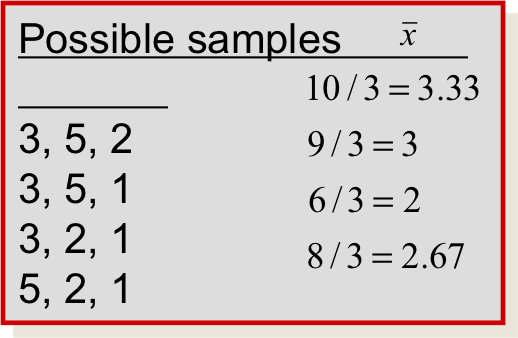
\includegraphics{sampling_pop.png} 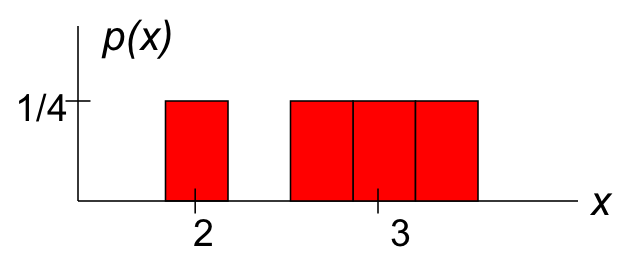
\includegraphics{sampling_pop1.png}

Each value of x-bar is equally likely, with probability 1/4

\subsection{Random Samples}\label{random-samples}

\begin{itemize}
\itemsep1pt\parskip0pt\parsep0pt
\item
  The sampling plan or experimental design determines the amount of
  information you can extract, and often allows you to measure the
  reliability of your inference.
\item
  Simple random sampling is a method of sampling that allows each
  possible sample of size n an equal probability of being selected.
\end{itemize}

\subsubsection{Types of Random Samples}\label{types-of-random-samples}

Sampling can occur in two types of practical situations:

\begin{itemize}
\itemsep1pt\parskip0pt\parsep0pt
\item
  Observational studies: The data existed before you decided to study
  it. Watch out for

  \begin{itemize}
  \itemsep1pt\parskip0pt\parsep0pt
  \item
    Nonresponse: Are the responses biased because only opinionated
    people responded? *Undercoverage: Are certain segments of the
    population systematically excluded?
  \item
    Wording bias: The question may be too complicated or poorly worded.
  \end{itemize}
\item
  Experimentation: The data are generated by imposing an experimental
  condition or treatment on the experimental units. *Hypothetical
  populations can make random sampling difficult if not impossible.

  \begin{itemize}
  \itemsep1pt\parskip0pt\parsep0pt
  \item
    Samples must sometimes be chosen so that the experimenter believes
    they are representative of the whole population.
  \item
    Samples must behave like random samples!
  \end{itemize}
\end{itemize}

\subsubsection{Examples}\label{examples}

\begin{itemize}
\itemsep1pt\parskip0pt\parsep0pt
\item
  Stratified random sample: Divide the population into sub populations
  or strata and select a simple random sample from each strata.
\item
  Cluster sample: Divide the population into subgroups called clusters;
  select a simple random sample of clusters and take a census of every
  element in the cluster.
\item
  1-in-k systematic sample: Randomly select one of the first k elements
  in an ordered population, and then select every k-th element
  thereafter.
\end{itemize}

\subsection{More Examples}\label{more-examples}

\begin{itemize}
\itemsep1pt\parskip0pt\parsep0pt
\item
  Divide California into counties and take a simple random sample within
  each county.

  \begin{itemize}
  \itemsep1pt\parskip0pt\parsep0pt
  \item
    Stratified
  \end{itemize}
\item
  Divide California into counties and take a simple random sample of 10
  counties.

  \begin{itemize}
  \itemsep1pt\parskip0pt\parsep0pt
  \item
    Clustered Divide a city into city blocks, choose a simple random
    sample of 10 city blocks, and interview all who live there.
  \item
    Clustered Choose an entry at random from the phone book, and select
    every 50th number thereafter.
  \item
    1 in 50 Systematic
  \end{itemize}
\end{itemize}

\subsection{Non-Random Sampling Plans: Not used for statistical
inference}\label{non-random-sampling-plans-not-used-for-statistical-inference}

\begin{itemize}
\item
  Can be used for data mining
\item
  Convenience sample: A sample that can be taken easily without random
  selection.

  \begin{itemize}
  \itemsep1pt\parskip0pt\parsep0pt
  \item
    People walking by on the street
  \end{itemize}
\item
  Judgment sample: The sampler decides who will and won't be included in
  the sample.\\
\item
  Quota sample: The makeup of the sample must reflect the makeup of the
  population on some selected characteristic.

  \begin{itemize}
  \itemsep1pt\parskip0pt\parsep0pt
  \item
    Race, ethnic origin, gender, etc.
  \end{itemize}
\end{itemize}

\subsection{Normal Curve (Outside Textbook
Information)}\label{normal-curve-outside-textbook-information}

\subsubsection{\ldots{}The Bell Shaped
Curve\ldots{}}\label{the-bell-shaped-curve}

The normal curve is symmetric, bell shaped, and asymptotic. The
inflection points fall at one standard deviation above and below the
mean.

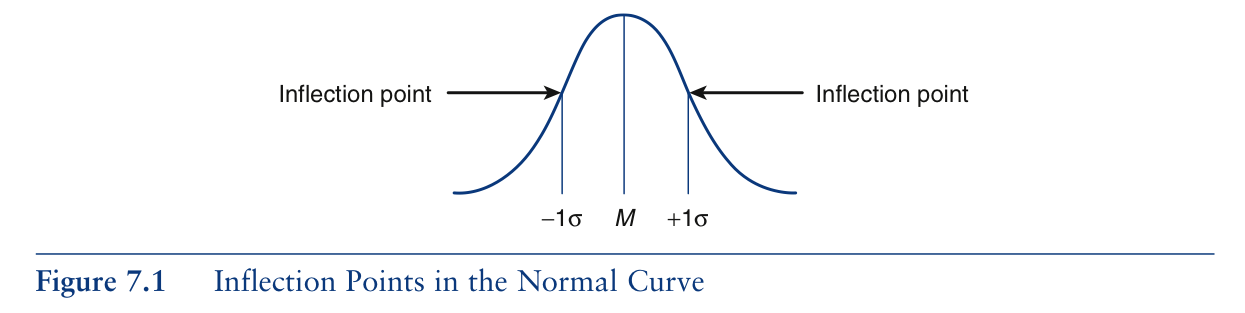
\includegraphics{normalcurve.png}

\subsection{Normal Curve: Areas Under the
Curve}\label{normal-curve-areas-under-the-curve}

The normal curve always has these proportions:

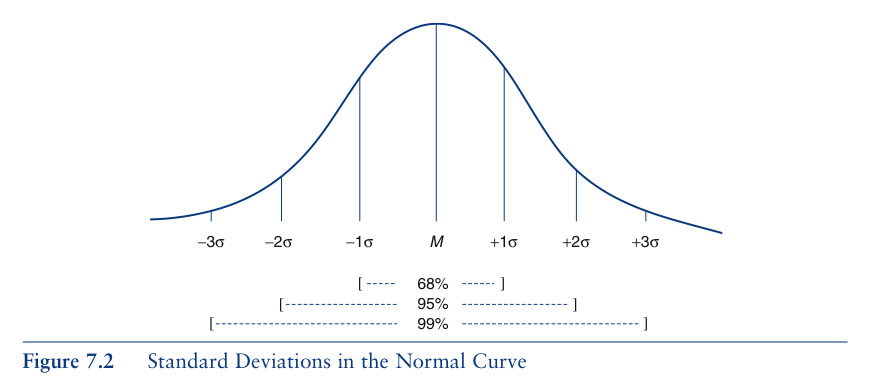
\includegraphics{normalcurveareas1.png}

and

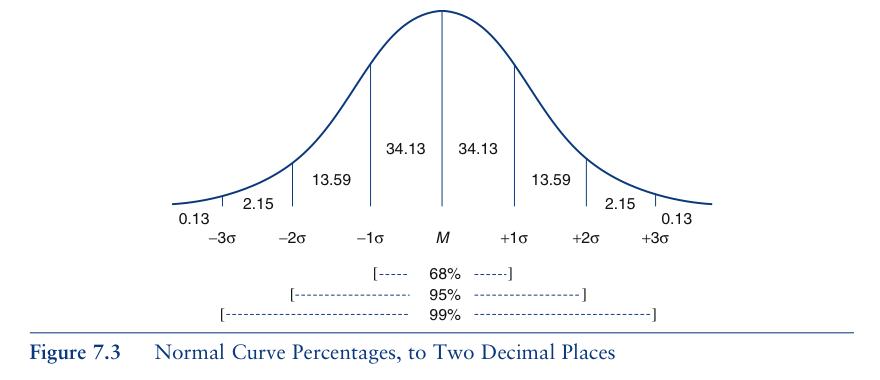
\includegraphics{normalcurveareas2.png}

\subsection{Hypotheses}\label{hypotheses}

Hypothesis tests follow a logical format \ldots{}

\begin{itemize}
\itemsep1pt\parskip0pt\parsep0pt
\item
  (𝑊ℎ𝑎𝑡 𝑑𝑖𝑑 𝑦𝑜𝑢 𝑔𝑒𝑡?−𝑊ℎ𝑎𝑡 𝑑𝑖𝑑 𝑦𝑜𝑢 𝑒𝑥𝑝𝑒𝑐𝑡?)/(𝑆𝑡𝑎𝑛𝑑𝑎𝑟𝑑𝑖𝑧𝑒𝑑 𝑅𝑎𝑛𝑑𝑜𝑚 𝐸𝑟𝑟𝑜𝑟 )
\end{itemize}

Z-scores have the same formula with X = what you got, M = what you
expected, and s = the standardized random error

\begin{itemize}
\itemsep1pt\parskip0pt\parsep0pt
\item
  Independent Variable (IV) -- the causal variable

  \begin{itemize}
  \itemsep1pt\parskip0pt\parsep0pt
  \item
    Is typically manipulated by the researcher
  \end{itemize}
\item
  Dependent Variable (DV) -- the effect

  \begin{itemize}
  \itemsep1pt\parskip0pt\parsep0pt
  \item
    Is typically expected to be impacted by the IV
  \end{itemize}
\item
  Extraneous Variable (XV) or Confounding Variable (CV) -- unintended
  variable

  \begin{itemize}
  \itemsep1pt\parskip0pt\parsep0pt
  \item
    Impacts the DV
  \end{itemize}
\item
  Hypotheses:

  \begin{itemize}
  \itemsep1pt\parskip0pt\parsep0pt
  \item
    Null Hypothesis -- no effect of IV on DV $\mu_x = \mu_y$
  \item
    Research (Alternative) Hypothesis (H1 or HA $\mu_x ≠ \mu_y$ or
    $\mu_x < \mu_y$) -- what is expected to be found
  \end{itemize}
\item
  Types of Hypotheses:

  \begin{itemize}
  \itemsep1pt\parskip0pt\parsep0pt
  \item
    Directional -- the IV is expected to ONLY increase or ONLY decrease
    the DV $\mu_x > \mu_y$ or $\mu_x < \mu_y$
  \item
    Nondirectional -- effect of IV could increas $\mu_x ≠ \mu_y$ or
    decrease the DV
  \end{itemize}
\end{itemize}

\subsection{Comparing Means}\label{comparing-means}

\begin{itemize}
\itemsep1pt\parskip0pt\parsep0pt
\item
  One Sample z test $z = \frac{\bar{x}-\mu}{\frac{\sigma}{\sqrt{n}}}$
\end{itemize}

\subsubsection{Work through Example Pg.
209}\label{work-through-example-pg.-209}

\subsubsection{Upcoming Items}\label{upcoming-items}

\begin{itemize}
\itemsep1pt\parskip0pt\parsep0pt
\item
  Two Sample z test (next chapter)
\item
  Multiple Samples (future chapters)
\end{itemize}

\subsection{Test Statistic: z score}\label{test-statistic-z-score}

Obtain the value for the test statistic that was calculated\ldots{} Page
561 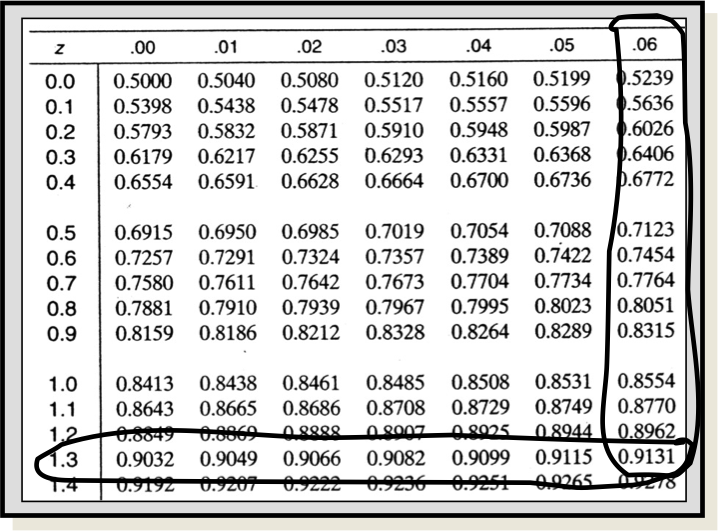
\includegraphics{ztable1.png}

It actually looks like this: 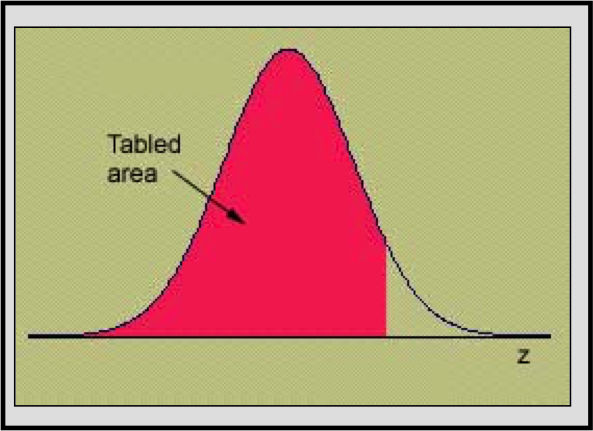
\includegraphics{zcurve.png}

For this value it would: 
\includegraphics{zarea.png}

Z-scores can be used to determine proportions of the curve

\subsection{Probabilities, Significance and
Confidence}\label{probabilities-significance-and-confidence}

For Critical Values of Z

\begin{longtable}[c]{@{}lll@{}}
\toprule\addlinespace
Prob. significance level & 1-tailed (directional) & 2-Tailed
(non-directional)
\\\addlinespace
\midrule\endhead
0.05 & 1.65 & 1.96
\\\addlinespace
0.01 & 2.33 & 2.58
\\\addlinespace
0.001 & 3.09 & 3.29
\\\addlinespace
\bottomrule
\end{longtable}

\textbf{Example: Pg. 212}

$z_{obtained}=\frac{51.70-50}{\frac{10}{\sqrt{100}}}$
$= \frac{1.70}{\frac{10}{10}} = \frac{1.70}{1} = 1.70$

Depending on the direction or non-direction of your result, you can make
the following conclusions if:

\begin{itemize}
\itemsep1pt\parskip0pt\parsep0pt
\item
  $z_{obt} > z_{crit}$ Reject the $H_0$ in favor of the $H_1$
\end{itemize}

and

\begin{itemize}
\itemsep1pt\parskip0pt\parsep0pt
\item
  $z_{obt} < z_{crit}$ Retain the $H_0$ in favor of the $H_1$
\end{itemize}

\subsection{Decision Making}\label{decision-making}

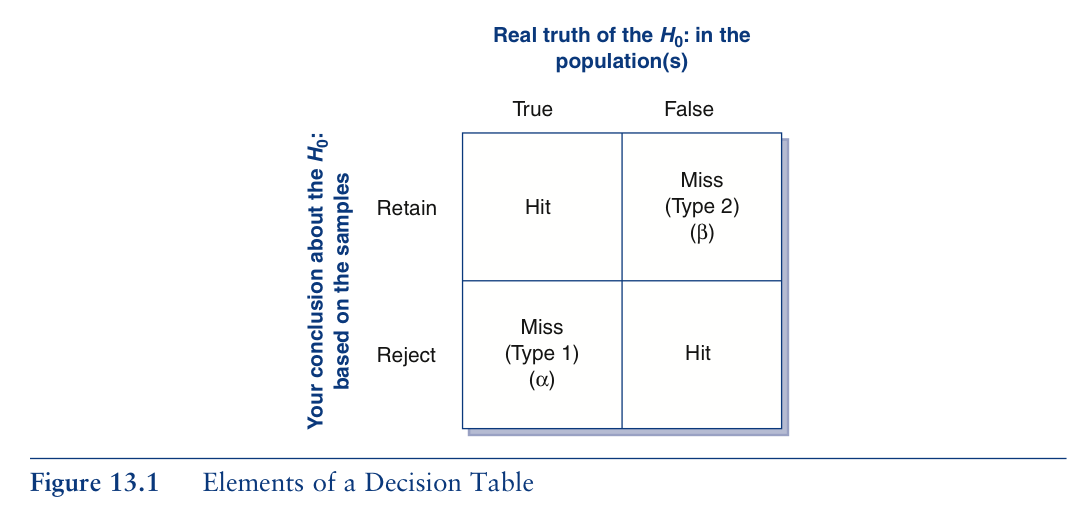
\includegraphics{decisions1.png}

\subsection{Types of Errors}\label{types-of-errors}

\subsubsection{Graphically}\label{graphically}

\begin{itemize}
\itemsep1pt\parskip0pt\parsep0pt
\item
  When the null is retained we expect the following to be the case
\end{itemize}

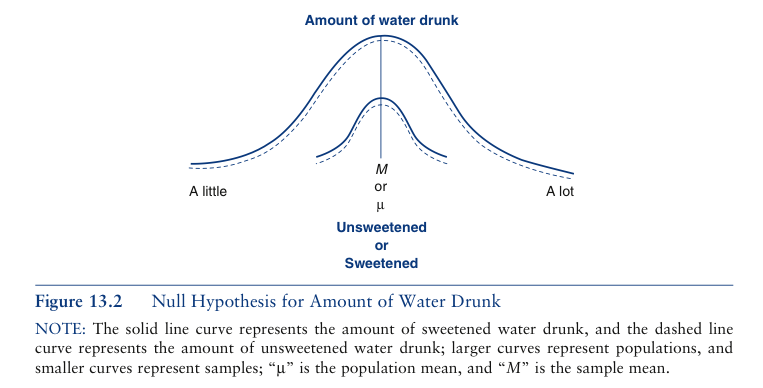
\includegraphics{error1.png}

\begin{itemize}
\itemsep1pt\parskip0pt\parsep0pt
\item
  When the null is rejected we expect the following to be the case
\end{itemize}

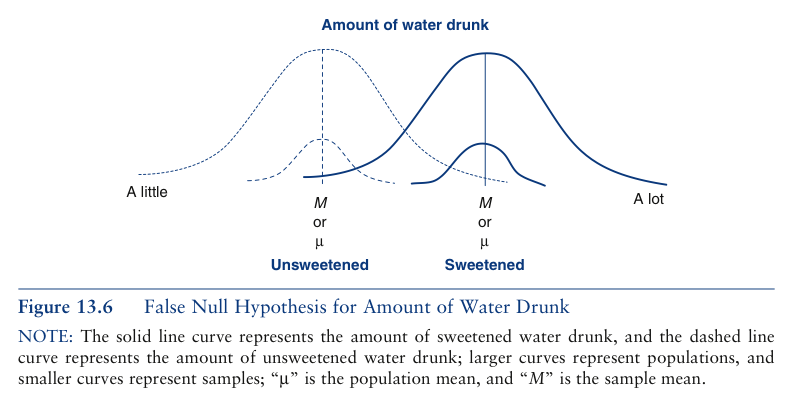
\includegraphics{error2.png}

\subsection{Types of Errors}\label{types-of-errors-1}

\subsubsection{Type I: $\alpha$ Error}\label{type-i-alpha-error}

\begin{enumerate}
\def\labelenumi{\arabic{enumi}.}
\itemsep1pt\parskip0pt\parsep0pt
\item
  The probability of falsely rejeting a true null hypothesis.
\item
  A type 1 error occurs when two samples appear to be different, but are
  actually from the same population.
\end{enumerate}

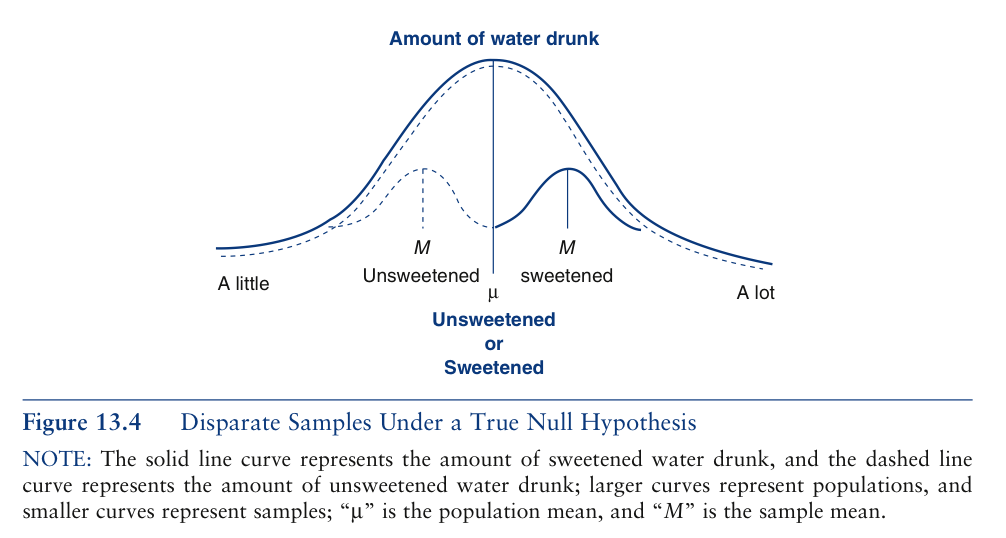
\includegraphics{type1.png}

\subsubsection{Type II: $\beta$ Error}\label{type-ii-beta-error}

\begin{enumerate}
\def\labelenumi{\arabic{enumi}.}
\itemsep1pt\parskip0pt\parsep0pt
\item
  Failure to reject a false null hypothesis.
\item
  Type 2 errors occur when two samples appear to be from the same
  population, but are actually from different populations.
\end{enumerate}

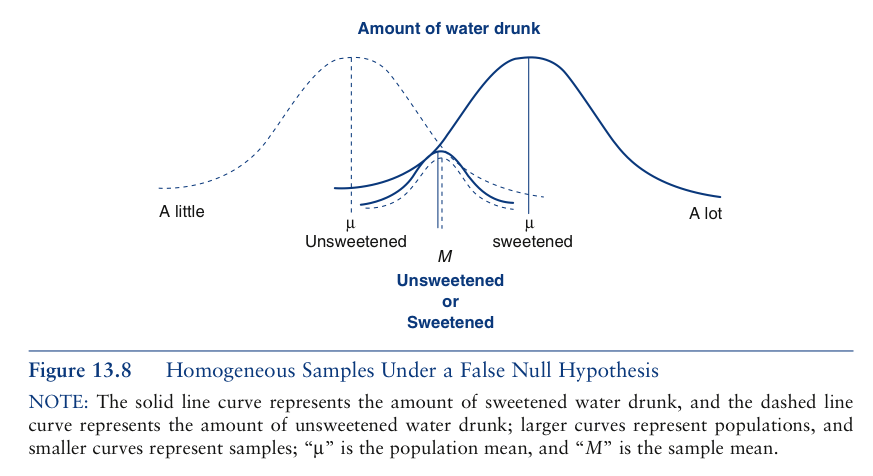
\includegraphics{type2.png}

\subsection{Equations: Population
Parameters}\label{equations-population-parameters}

Equations calculated \textbf{FOR POPULATION MEASURES} only.

\begin{itemize}
\itemsep1pt\parskip0pt\parsep0pt
\item
  The Mean: $\mu =\frac{\Sigma x}{N}$
\item
  Variance (computational): $\sigma ^2 = \frac{\Sigma(x - \mu)^2}{N}$
\item
  Variance (definitional):
  $\sigma^2 = \frac{\Sigma x^2 - \frac{(\Sigma x)^2}{N}}{N}$
\item
  Standard Deviation: $\sqrt{\sigma^2} = \sigma$
\end{itemize}

\subsection{Equations: Sample
Statistics}\label{equations-sample-statistics}

Equations calculated for \textbf{SAMPLE MEASURES} only

\begin{itemize}
\itemsep1pt\parskip0pt\parsep0pt
\item
  The Mean: $\bar{x} = \frac{\Sigma x}{n}$
\item
  Variance (computational): $s^2 = \frac{\Sigma (x - \bar{x})^2}{n}$
\item
  Variance (definitional):
  $s^2 = \frac{\Sigma x^2 - \frac{(\Sigma x)^2}{n}}{n}$
\item
  Standard Deviation: $\sqrt{s^2} = s$
\end{itemize}

\subsubsection{New Equation: z Test of Statistical
Significance}\label{new-equation-z-test-of-statistical-significance}

The z test equation is:
$z = \frac{\bar{x}-\mu}{\frac{\sigma}{\sqrt{n}}}$

\subsection{Key Concepts}\label{key-concepts}

\begin{itemize}
\itemsep1pt\parskip0pt\parsep0pt
\item
  Tests of Statistical Significance

  \begin{itemize}
  \itemsep1pt\parskip0pt\parsep0pt
  \item
    Techniques that help us to generalize to a larger group.
  \end{itemize}
\item
  Inferential Statistics (Inductive Statistics)

  \begin{itemize}
  \itemsep1pt\parskip0pt\parsep0pt
  \item
    The body of knowledge that deals with tests of significance.
  \end{itemize}
\item
  Descriptive Statistics

  \begin{itemize}
  \itemsep1pt\parskip0pt\parsep0pt
  \item
    Statistics in which frequency distributions or relationships between
    variables are described.
  \end{itemize}
\item
  Population/Sampling Universe

  \begin{itemize}
  \itemsep1pt\parskip0pt\parsep0pt
  \item
    The group about which we want to generalize.
  \end{itemize}
\item
  Sample

  \begin{itemize}
  \itemsep1pt\parskip0pt\parsep0pt
  \item
    The smaller group from the population that is selected to be
    studied.
  \end{itemize}
\item
  Drawing a Sample

  \begin{itemize}
  \itemsep1pt\parskip0pt\parsep0pt
  \item
    The selection of subjects to be in a sample.
  \end{itemize}
\item
  Sampling Bias/Biased Sample

  \begin{itemize}
  \itemsep1pt\parskip0pt\parsep0pt
  \item
    The mechanism for selecting the sample that causes the sample to be
    not representative of the population as a whole.
  \end{itemize}
\item
  Random Sample

  \begin{itemize}
  \itemsep1pt\parskip0pt\parsep0pt
  \item
    A sample that is not biased.
  \end{itemize}
\item
  Simple Random Sample

  \begin{itemize}
  \itemsep1pt\parskip0pt\parsep0pt
  \item
    A sample drawn in such a way that every member of the population has
    an equal likelihood of being included in the sample.
  \end{itemize}
\item
  Sampling Error

  \begin{itemize}
  \itemsep1pt\parskip0pt\parsep0pt
  \item
    A deviation from what actually exists in the population not
    associated with sampling bias but still existing, even though the
    sample was randomly drawn.
  \end{itemize}
\item
  Normal Curve

  \begin{itemize}
  \itemsep1pt\parskip0pt\parsep0pt
  \item
    The normal curve is symmetric, bell shaped, and asymptotic. The
    inflection points fall at one standard deviation above and below the
    mean.
  \end{itemize}
\item
  Hypotheses

  \begin{itemize}
  \itemsep1pt\parskip0pt\parsep0pt
  \item
    Null Hypothesis ($H_0$): A statement postulating that in the
    population, the means of two or more groups are the same or, in the
    case of two variables in a cross-tabulation, that in the population,
    the two variables are unrelated.\\
  \item
    Alternative/Research Hypothesis ($H_1$): Statement that indicates
    that in the population, the means of two or more groups differ or,
    in the case of a cross-tabulation, the two variables are related.
  \end{itemize}
\item
  Fallacy of Affirming the Consequent

  \begin{itemize}
  \itemsep1pt\parskip0pt\parsep0pt
  \item
    A principle of logic that suggests that the only way to ``prove''
    the alternative or research hypothesis is to demonstrate that the
    null hypothesis is true.
  \end{itemize}
\item
  Chi-Square Test

  \begin{itemize}
  \itemsep1pt\parskip0pt\parsep0pt
  \item
    A test of significance for two variables in a cross-tabulation.
  \end{itemize}
\item
  Sample Statistics

  \begin{itemize}
  \itemsep1pt\parskip0pt\parsep0pt
  \item
    Information computed from sample data.
  \end{itemize}
\item
  Population Parameters

  \begin{itemize}
  \itemsep1pt\parskip0pt\parsep0pt
  \item
    Information computed from population data.
  \end{itemize}
\item
  Population mean, mu, and $\mu$

  \begin{itemize}
  \itemsep1pt\parskip0pt\parsep0pt
  \item
    Population Mean: $\mu$ is the population's mean
  \end{itemize}
\item
  Population Standard Deviation / lower case sigma $\sigma$

  \begin{itemize}
  \itemsep1pt\parskip0pt\parsep0pt
  \item
    Population St.~Deviation: $\sigma^2$ is the population's standard
    deviation
  \end{itemize}
\item
  N:

  \begin{itemize}
  \itemsep1pt\parskip0pt\parsep0pt
  \item
    Population size.
  \end{itemize}
\item
  One Sample Tests

  \begin{itemize}
  \itemsep1pt\parskip0pt\parsep0pt
  \item
    Tests that compare data from a sample to similar data in a
    population.
  \end{itemize}
\item
  One Sample z test.

  \begin{itemize}
  \itemsep1pt\parskip0pt\parsep0pt
  \item
    A test of significance that can be performed when we know the
    population's standard deviation as well as it's mean.
  \end{itemize}
\item
  One Sample t test

  \begin{itemize}
  \itemsep1pt\parskip0pt\parsep0pt
  \item
    A test that can be performed when we know the population's mean but
    not it's standard deviation.
  \end{itemize}
\item
  Two Sample t test A t test that compares two sample means, rather than
  one sample's mean to another population's mean.
\item
  One Way Analysis of Variance (ANOVA)

  \begin{itemize}
  \itemsep1pt\parskip0pt\parsep0pt
  \item
    A test in which two or more sample means may be compared
    simultaneously.
  \end{itemize}
\item
  .05 Level of Significance

  \begin{itemize}
  \itemsep1pt\parskip0pt\parsep0pt
  \item
    The probability level classically used by social statisticians for
    determining that a null hypothesis may be rejected.
  \end{itemize}
\item
  Probabilities

  \begin{itemize}
  \itemsep1pt\parskip0pt\parsep0pt
  \item
    Proportions that reflect the likelihood of a particular outcome.
  \end{itemize}
\item
  Type I Error / Alpha ($\alpha$) Error

  \begin{itemize}
  \itemsep1pt\parskip0pt\parsep0pt
  \item
    The probability of falsely rejecting a true null hypothesis.
  \end{itemize}
\item
  Non-directional Hypothesis / Two-tailed Alternative Hypothesis /
  Two-tailed Test

  \begin{itemize}
  \itemsep1pt\parskip0pt\parsep0pt
  \item
    An alternative hypothesis that does not specify the directionality
    (i.e.~which mean will ultimately be larger).
  \end{itemize}
\item
  Directional Hypothesis / One-tailed Alternative Hypothesis /
  One-tailed Test

  \begin{itemize}
  \itemsep1pt\parskip0pt\parsep0pt
  \item
    An alternative hypothesis that does specify which mean will be the
    larger one.
  \end{itemize}
\item
  Degrees of Freedom:

  \begin{itemize}
  \itemsep1pt\parskip0pt\parsep0pt
  \item
    An additional piece of information needed for tests where critical
    values vary with the problem and may be functions of such things as
    sample size.
  \end{itemize}
\item
  Type II Error/ Beta ($\beta$) Error

  \begin{itemize}
  \itemsep1pt\parskip0pt\parsep0pt
  \item
    Failure to reject a false null hypothesis.
  \end{itemize}
\end{itemize}

\subsection{Next Time}\label{next-time}

\begin{itemize}
\itemsep1pt\parskip0pt\parsep0pt
\item
  Wednesday: Chapter 8 Probability, z and t tests
\item
  IMPORTANT DEADLINES:

  \begin{itemize}
  \itemsep1pt\parskip0pt\parsep0pt
  \item
    Homework 1 is due by -- Midnight 9/30/14. Late fee kicks in after
    midnight.
  \end{itemize}
\item
  Upcoming Items:

  \begin{itemize}
  \itemsep1pt\parskip0pt\parsep0pt
  \item
    Homework 2 released next Monday 10/6/14
  \item
    Exam 2 10/22
  \item
    Writing Draft 10/29
  \end{itemize}
\end{itemize}

\end{document}
